\documentclass[a4paper]{article}

%% Language and font encodings
\usepackage[english]{babel}
\usepackage[utf8x]{inputenc}
\usepackage[T1]{fontenc}

%% Sets page size and margins
\usepackage[a4paper,top=3cm,bottom=2cm,left=3cm,right=3cm,marginparwidth=1.75cm]{geometry}

%% Useful packages
\usepackage{amsmath}
\usepackage{subcaption}
\usepackage{graphicx}
\usepackage[colorinlistoftodos]{todonotes}
\usepackage[colorlinks=true, allcolors=blue]{hyperref}

\title{ECE 276A Homework 1}
\author{Samuel Bauza}

\begin{document}
\maketitle

\section{Introduction}

	Automatic image segmentation is a topic of interest to a wide range of fields. Intelligent vehicles require may use image segmentation to detect hazards in their surroundings, while drones might use it to focus on regions of interest. In particular, autonomous robots on the outer planets could likely require some form of autonomy as communication delays prevent real-time action by ground control.
    
	This paper goes into one potential method of detecting the presence of a red barrel among a varied background. The data is approximated as a multi-variate gaussian, and bayes rule is used to estimate the relative probabilities of various classes. Blob morphology is used to clean up the resulting map, and linear regression is used to estimate the distance from camera to the barrel.
    
	Decent results were achieved when the barrel is well lit and is not adjacent to similarly colored objects. The model was not complex enough to account for reflections or other smooth red objects.


\section{Problem Formulation}

	The barrel detection can be broken down into several parts: segmentation, mask processing, and object scoring. More detailed information about each step is contained in the Technical Approach section.
    
	Segmentation is the process of guessing what pixels of an image belong to a class. For this project, we segmented solely based on color. Segmentation could also be done on local spectral content, possibly distinguishing the smooth barrel from more textured background objects. In this case. the determination of what class a pixel belongs to is done using Bayes rule of probability modeling.
    
	Mask processing takes the segmented image and applies several blob morphological operations to remove small noise blobs, and help connect touching blobs. Erode and dilate are used in combination to achieve this effect.
    
	Finally, barrel scoring helps select blobs that best match the typical profile of a red barrel. This is achieved by examining the general shape attributes of each blob. Objects that sufficiently match the profile of a barrel are then indicated and presented to the user.


\subsection{Technical Information}

As previously mentioned, Bayes rule (EQ. \ref{eq:Bayes_rule}) is used to compare relative probabilities that a pixel belongs to a class. The prior probability (EQ. \ref{eq:prior_ratio}) is modeled by counting the occurrences of pixels in each class, and the posterior probability (EQ. eq:\ref{gauss_pdf}) is modeled by a multivariate gaussian distribution. Each value of the distribution is a vector of 3 components, made up of the color channels of each pixel. This color mode is easily configurable to allow for testing different modes (RGB / HSV etc.).

\begin{equation*}\label{eq:Bayes_rule}
P(y | \boldsymbol{x_i}) = \dfrac{P(\boldsymbol{x_i}|y)P(y)}{P(\boldsymbol{x_i})}
\end{equation*}

\begin{equation*}\label{eq:prior_ratio}
P_Y(\boldsymbol{Y}) = 
\dfrac{N pixels in labeled as class}{N labeled pixels}
\end{equation*}

\begin{equation*}\label{eq:gauss_pdf}
P_X(\boldsymbol{x})=\frac{1}{\sqrt{(2\pi)^n|\boldsymbol\Sigma|}}
\exp\left(-\frac{1}{2}(\boldsymbol{x}-{\mu})^T{\boldsymbol\Sigma}^{-1}(\boldsymbol{x}-{\mu})
\right)
\end{equation*}

	The first step in the process is to collect the data sets and generate class distributions. Images initially look like Figure \ref{fig:init_image}. Using training images paired with data masks, a Nx3 matrix is generated for each class, where N is the number of data samples in that class. The mean and covariance matrices (EQ. \ref{eq:mean}) for each class are calculated using these data sets. The result should be a 1x3 mean vector, and a 3x3 covariance matrix for each class.
    
\begin{equation*}\label{eq:mean}
\mu_i = x_i^T * x_i 
\end{equation*}
\begin{equation*}
Cov(X) = x^T * X
\end{equation*}
 
	These terms are used to calculate the class probability in Bayes rule. Because only the class with the highest probability is selected, the log likelihood can be used, simplifying some of the calculations. Calculation of the exponential term is optimized to improve timing and memory performance, only the diagonals terms are calculated.
    
	At this point, each pixel is associated with a particular class, resulting with a labeled image similar to Figure \ref{fig:segmented_image}. The non-barrel classes are set to 0, resulting in a barrel mask Figure \ref{fig:mask_image}. Blob morphology is a method of tweaking a mask to expand or contract various regions, examples of this and the kernels used to achieve it are in (Figure \ref{fig:dilate_mask}, \ref{fig:erode_mask} ). This process helps remove small groups of barrel-labeled pixels, and fills in large regions. After several stages of this small regions are removed and the resulting image should look similar to Figure \ref{fig:morph_image}.
    
	Finally, a method of calculating the ‘barrelness’ is used to determine what blobs are most likely to be barrels vs. other objects. The scoring system is very rudimentary, and takes into account two measurements, the solidarity (Pixels used in box / pixels in box) and aspect ratio (barrel width / height). Because barrels may be partially obscured by other objects, the resulting blobs may be disjoint. To account for this, combinations of the present blobs Figure \ref{fig:labeled_image} should be examined and tested for barrelness. Currently, all combinations of length 1 to 4 are tested for barrelness.
    
	At this point, a minimum area rectangle is drawn on the original image, and its location and score are displayed. At this point, the image will appear similar to Figure \ref{fig:ident_image}.

\section{Results}

A sampling of interesting training results are in (Figures \ref{fig:train0}-\ref{fig:train3}). The test results and their respective detected corners are in (Figures \ref{fig:test0}-\ref{fig:test9}). Within minimal tweaking, the algorithm was able to detect barrels in most cases in the test set. It has significant difficulty when adjacent to objects that are of a very similar color to the barrel (reflections / coke sign), however it is quite adept at connecting barrel segments that are separated by obstructions (stairs / railing). The resulting distance estimate

\begin{table}
\centering
\begin{tabular}{|c|c|c|c|}
Image & Barrelness & Bounds & Distance \\\hline
ImageNo[01] & .43 & [362,557,526,666] & 6.68 \\
ImageNo[02] & .25 & [459,591,513,647] & 6.69\\
ImageNo[03] & .20 & [765,798,816,877] & 6.69\\
ImageNo[03] & .10 & [82,627,537,913]  & 6.68\\
ImageNo[04] & .17 & [266,470,627,802] & 6.67\\
ImageNo[05] & .39 & [404,604,519,685] & 6.67\\
ImageNo[06] & .24 & [179,318,716,955] & 6.68\\
ImageNo[07] & .46 & [106,603,192,660] & 6.65\\
ImageNo[08] & .07 & [217,520,503,712] & 6.68\\
ImageNo[09] & .29 & [565,626,708,694] & 6.68\\
ImageNo[10] & .44 & [230,622,308,676] & 6.69
\end{tabular}
\caption{\label{tab:bound_distance_table}Approximated barrel bound and distances.}
\end{table}

\begin{figure}[!tbp]
  \centering
  \begin{subfigure}[b]{.4\textwidth}
    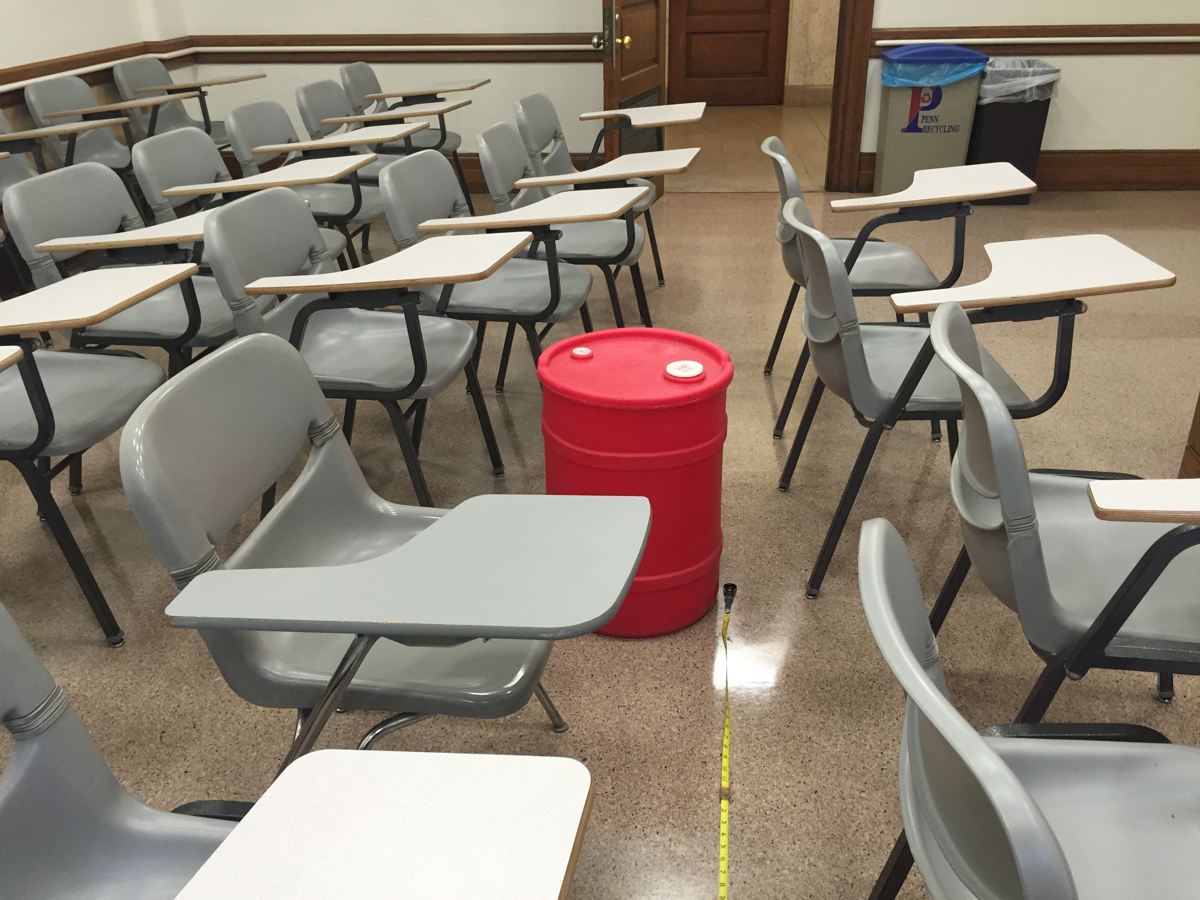
\includegraphics[width=1\textwidth]{2_3.png}
    \caption{\label{fig:init_image}Initial Image.}
  \end{subfigure}
  \begin{subfigure}[b]{.4\textwidth}
    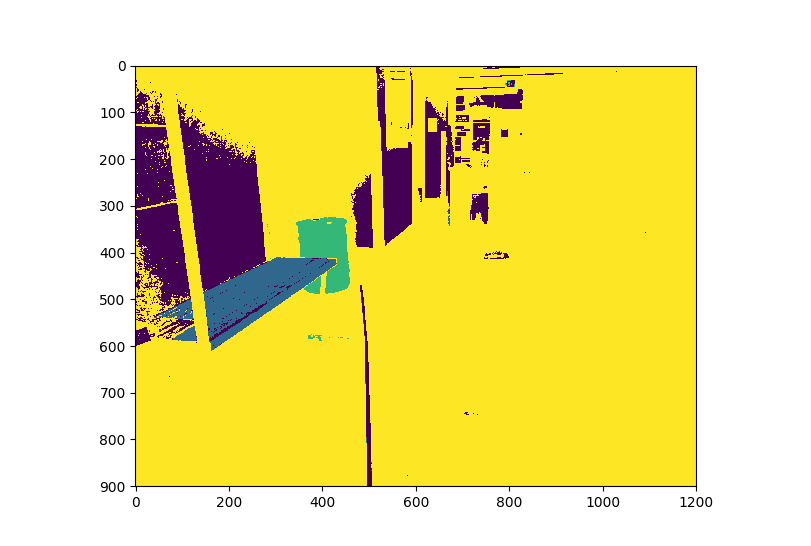
\includegraphics[width=1.3\textwidth]{segmented.png}
\caption{\label{fig:segmented_image}Image after gaussian classification.}
  \end{subfigure}
  \caption{\label{fig:first_set}}
\end{figure}

\begin{figure}[!tbp]
  \centering
  \begin{subfigure}[b]{.4\textwidth}
    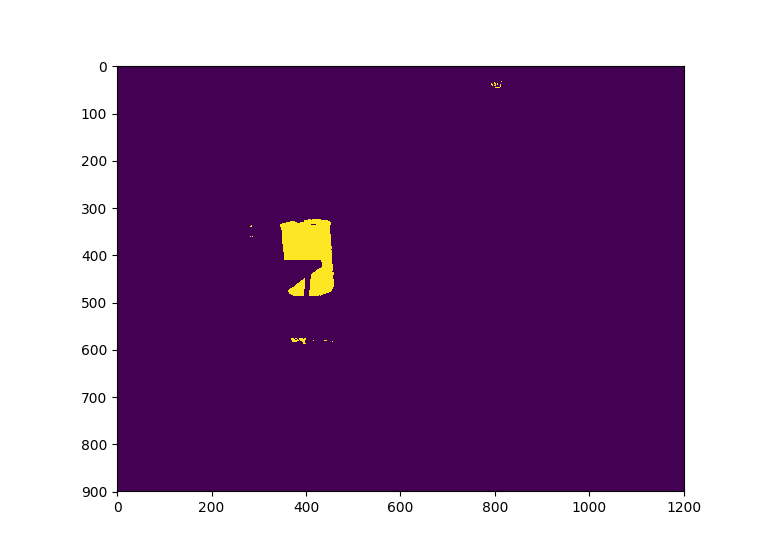
\includegraphics[width=1.3\textwidth]{barrel_mask.png}
\caption{\label{fig:mask_image}Mask of only barrel pixels.}
  \end{subfigure}
  \begin{subfigure}[b]{.4\textwidth}
    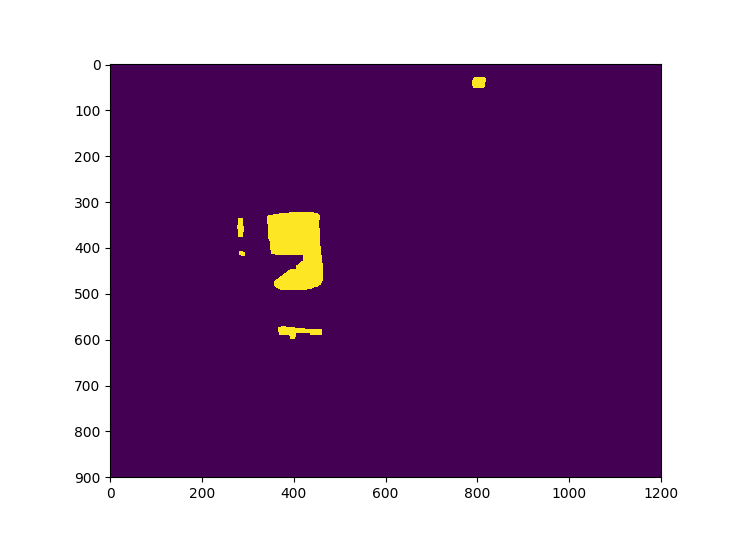
\includegraphics[width=1.3\textwidth]{Morphed_image.png}
\caption{\label{fig:morph_image}Post-morphology image.}
  \end{subfigure}
  \caption{\label{fig:second_set}}
\end{figure}

\begin{figure}[!tbp]
  \centering
  \begin{subfigure}[b]{.4\textwidth}
    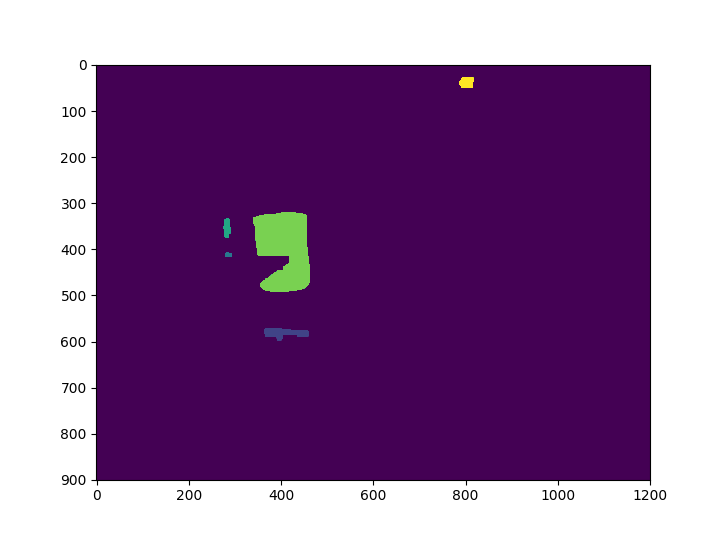
\includegraphics[width=1.3\textwidth]{labeled_image.png}
\caption{\label{fig:labeled_image}Connected components individually labeled.}
  \end{subfigure}
  \begin{subfigure}[b]{.4\textwidth}
    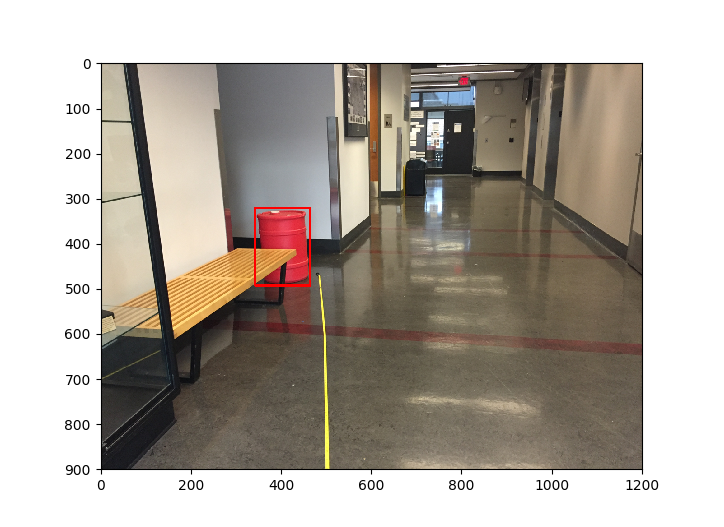
\includegraphics[width=1.3\textwidth]{drawn_barrel.png}
\caption{\label{fig:ident_image}Identified barrel with marked bounds.}
  \end{subfigure}
  \caption{\label{fig:third_set}}
\end{figure}

\begin{figure}[!tbp]
  \centering
  \begin{subfigure}[b]{.4\textwidth}
    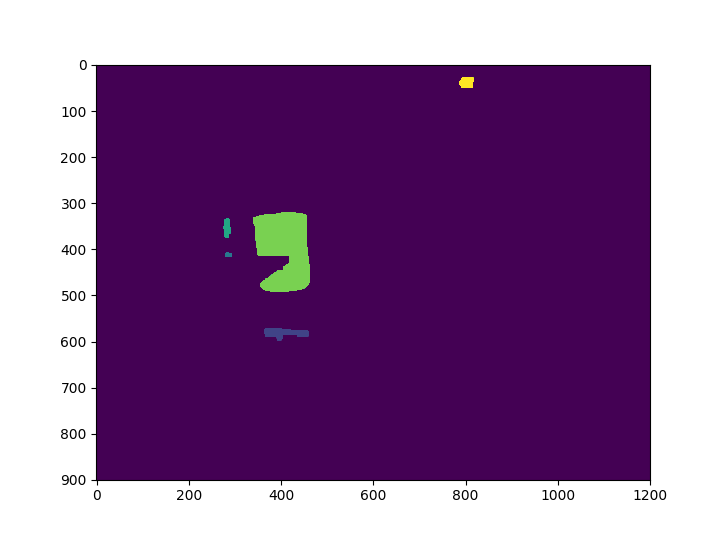
\includegraphics[width=1.3\textwidth]{labeled_image.png}
\caption{\label{fig:dilate_mask}Dilation mask.}
  \end{subfigure}
  \begin{subfigure}[b]{.4\textwidth}
    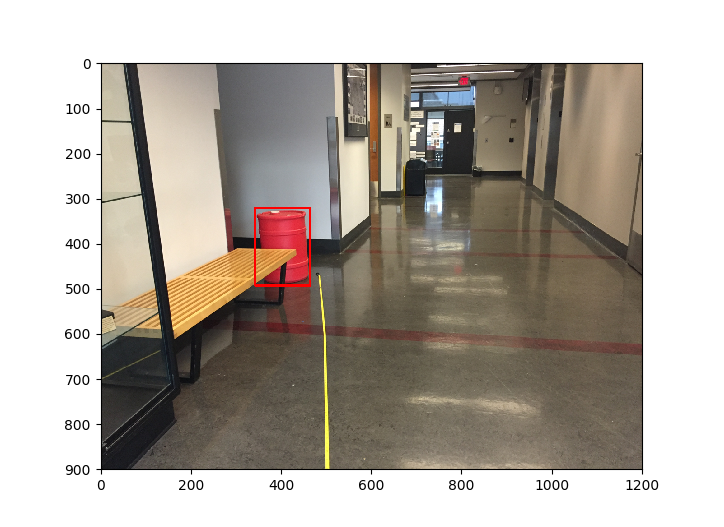
\includegraphics[width=1.3\textwidth]{drawn_barrel.png}
\caption{\label{fig:erode_mask}Erosion mask.}
  \end{subfigure}
  \caption{\label{fig:fourth_set}}
\end{figure}

\begin{figure}[!tbp]
  \centering
  \begin{subfigure}[b]{.4\textwidth}
    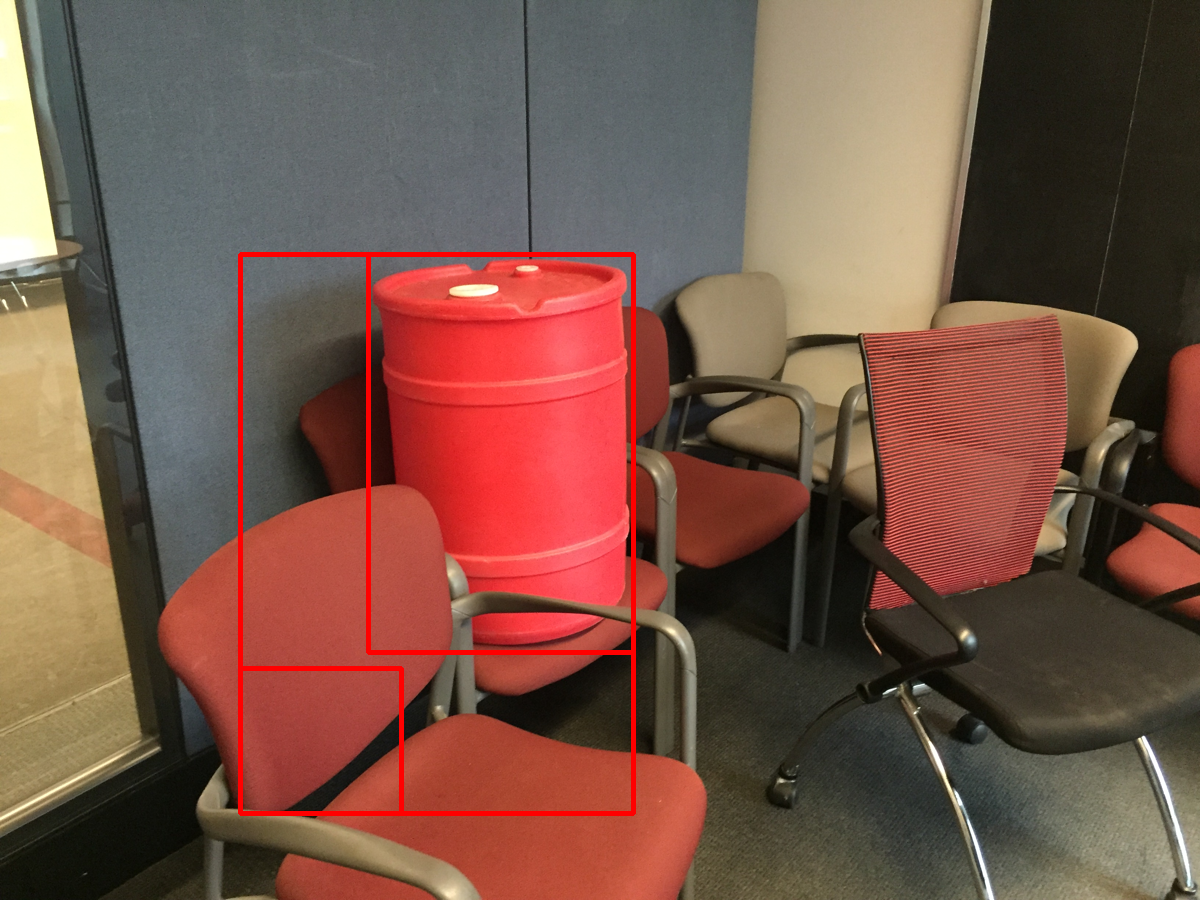
\includegraphics[width=1\textwidth]{train_image0.png}
\caption{\label{fig:train0}Training image 0 result.}
  \end{subfigure}
  \begin{subfigure}[b]{.4\textwidth}
    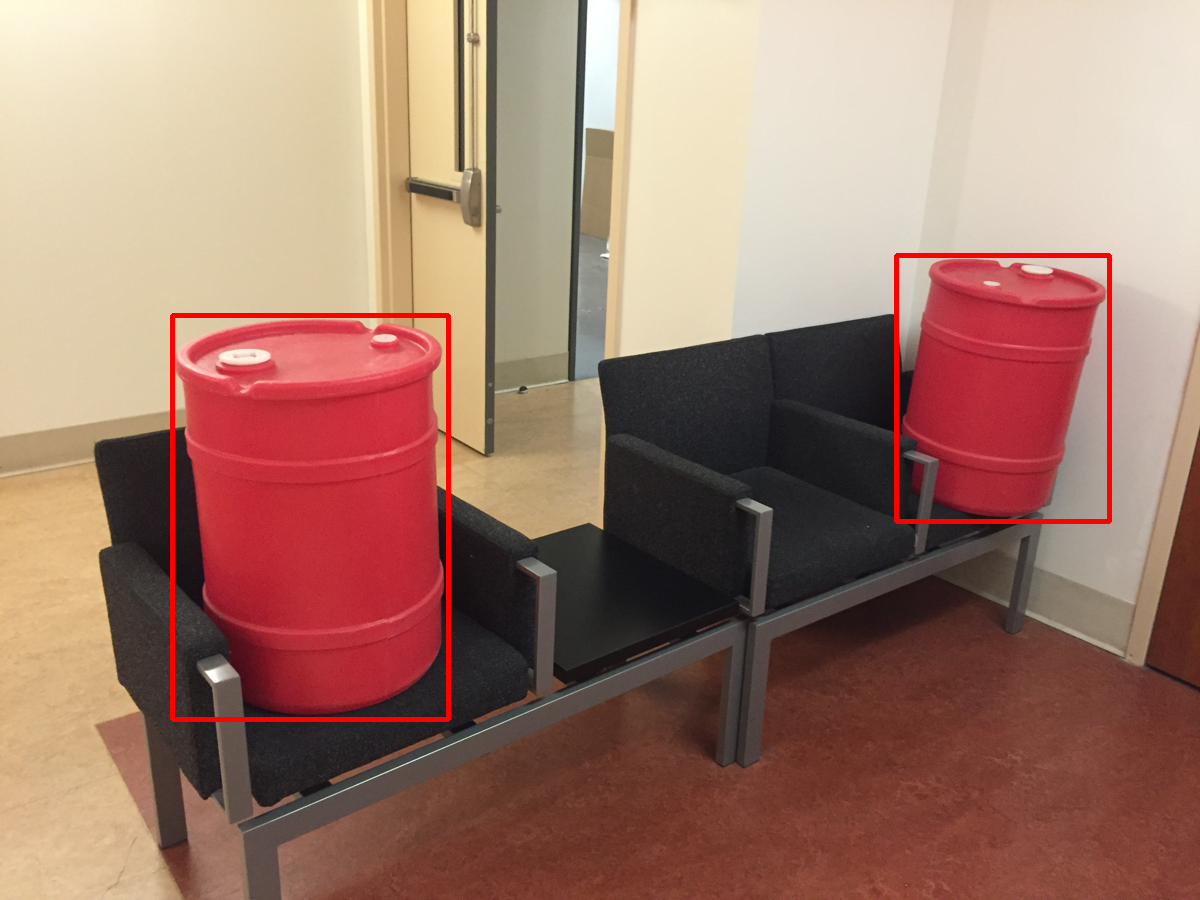
\includegraphics[width=1\textwidth]{train_image1.png}
\caption{\label{fig:train1}Training image 1 result.}
  \end{subfigure}
  \caption{\label{fig:train0_set}}
\end{figure}

\begin{figure}[!tbp]
  \centering
  \begin{subfigure}[b]{.4\textwidth}
    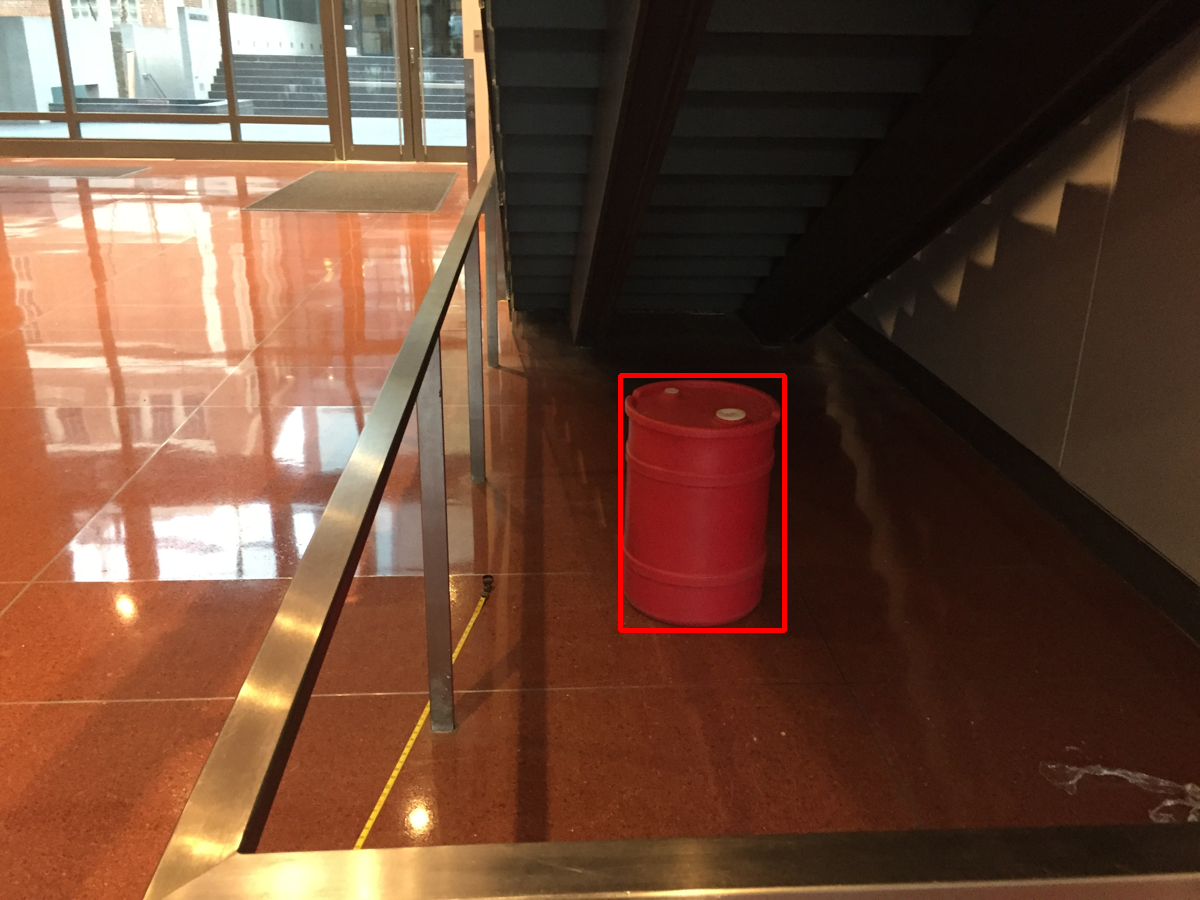
\includegraphics[width=1\textwidth]{train_image2.png}
\caption{\label{fig:train2}Training image 2 result.}
  \end{subfigure}
  \begin{subfigure}[b]{.4\textwidth}
    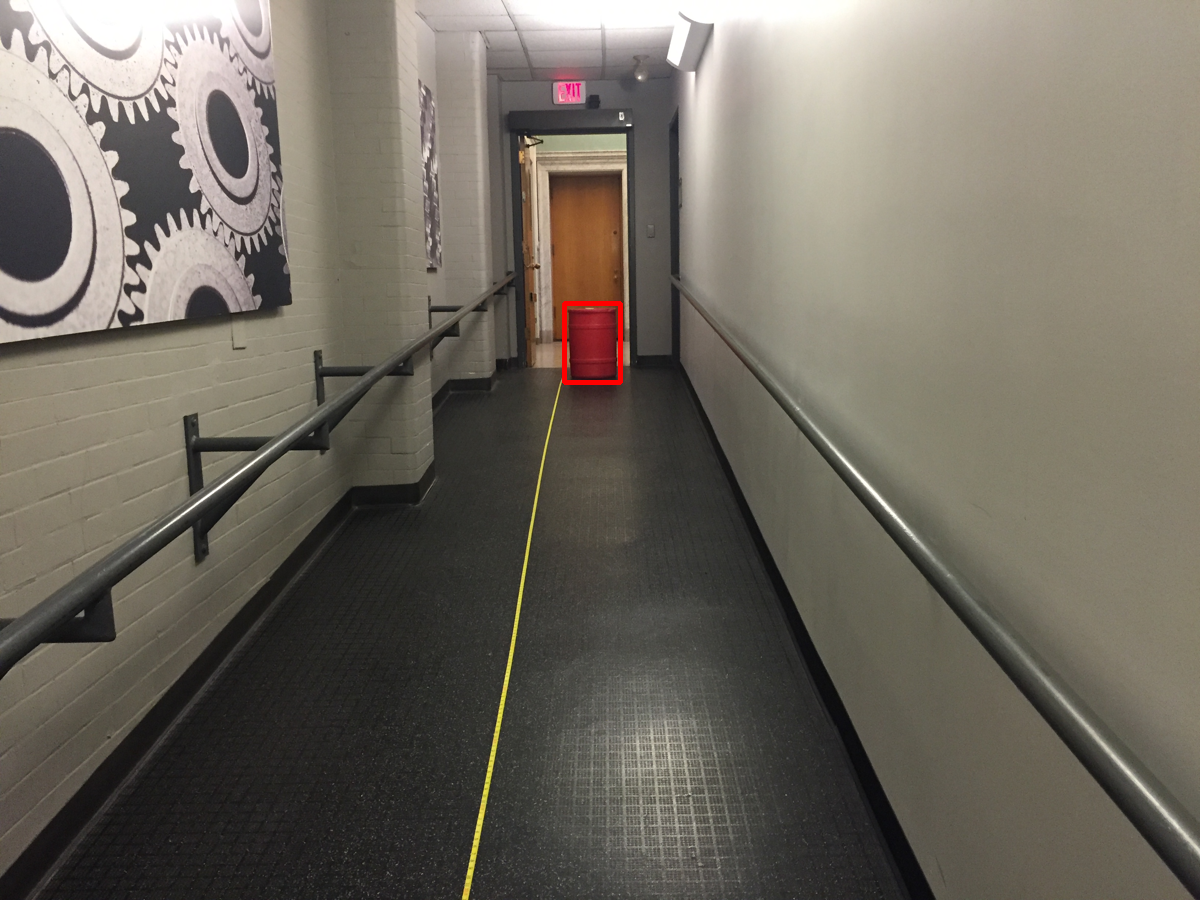
\includegraphics[width=1\textwidth]{train_image3.png}
\caption{\label{fig:train3}Training image 3 result.}
  \end{subfigure}
  \caption{\label{fig:train1_set}}
\end{figure}

\begin{figure}[!tbp]
  \centering
  \begin{subfigure}[b]{.4\textwidth}
    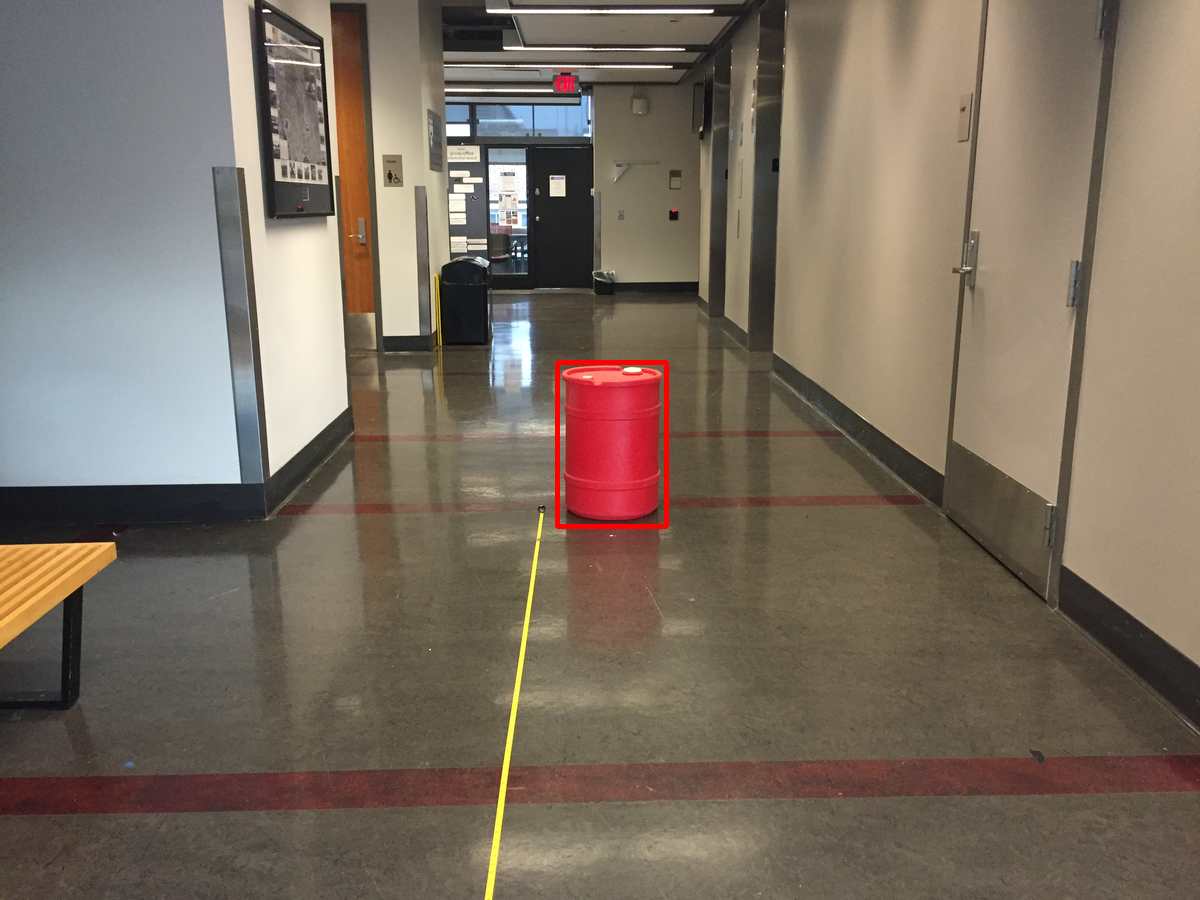
\includegraphics[width=1\textwidth]{test_image0.png}
\caption{\label{fig:test0}Test image 0 result.}
  \end{subfigure}
  \begin{subfigure}[b]{.4\textwidth}
    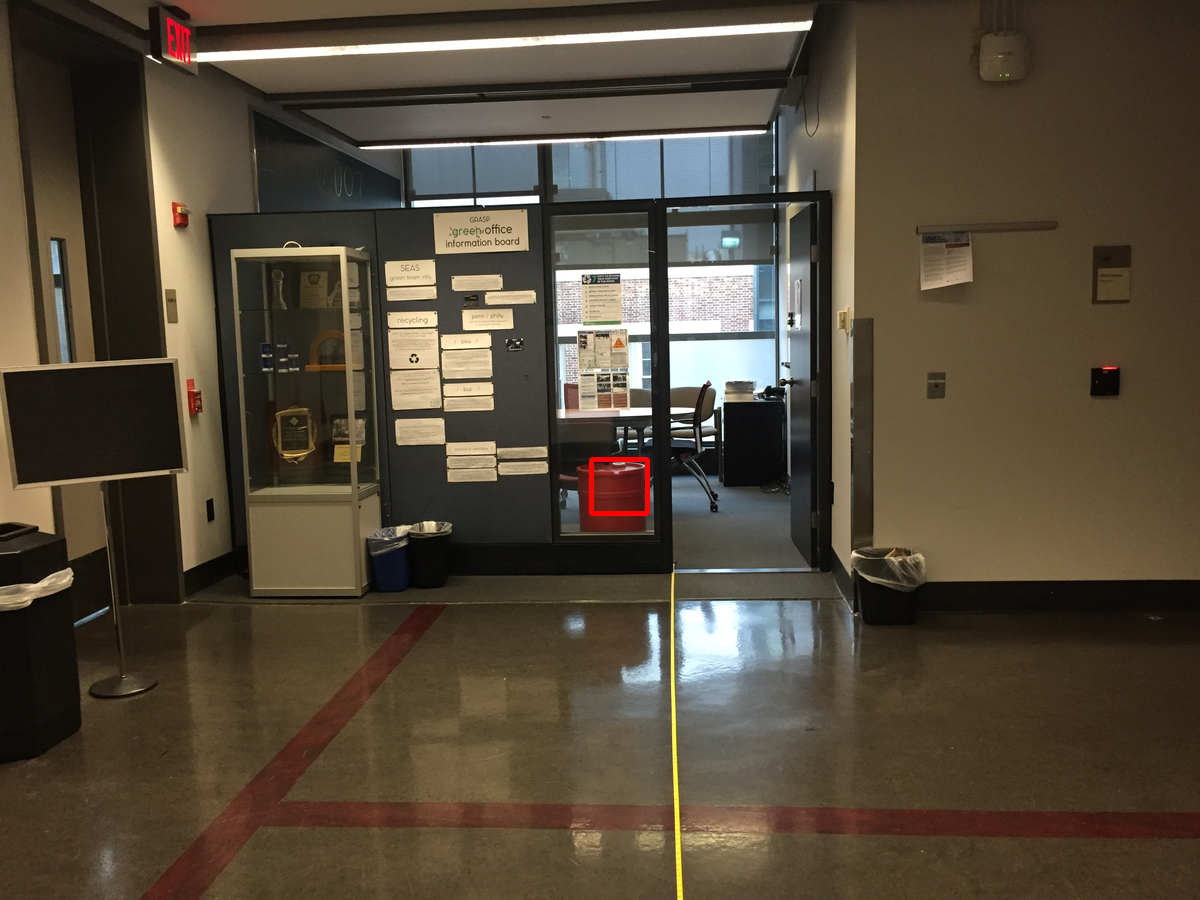
\includegraphics[width=1\textwidth]{test_image1.png}
\caption{\label{fig:test1}Test image 1 result.}
  \end{subfigure}
  \caption{\label{fig:test1_set}}
\end{figure}

\begin{figure}[!tbp]
  \centering
  \begin{subfigure}[b]{.4\textwidth}
    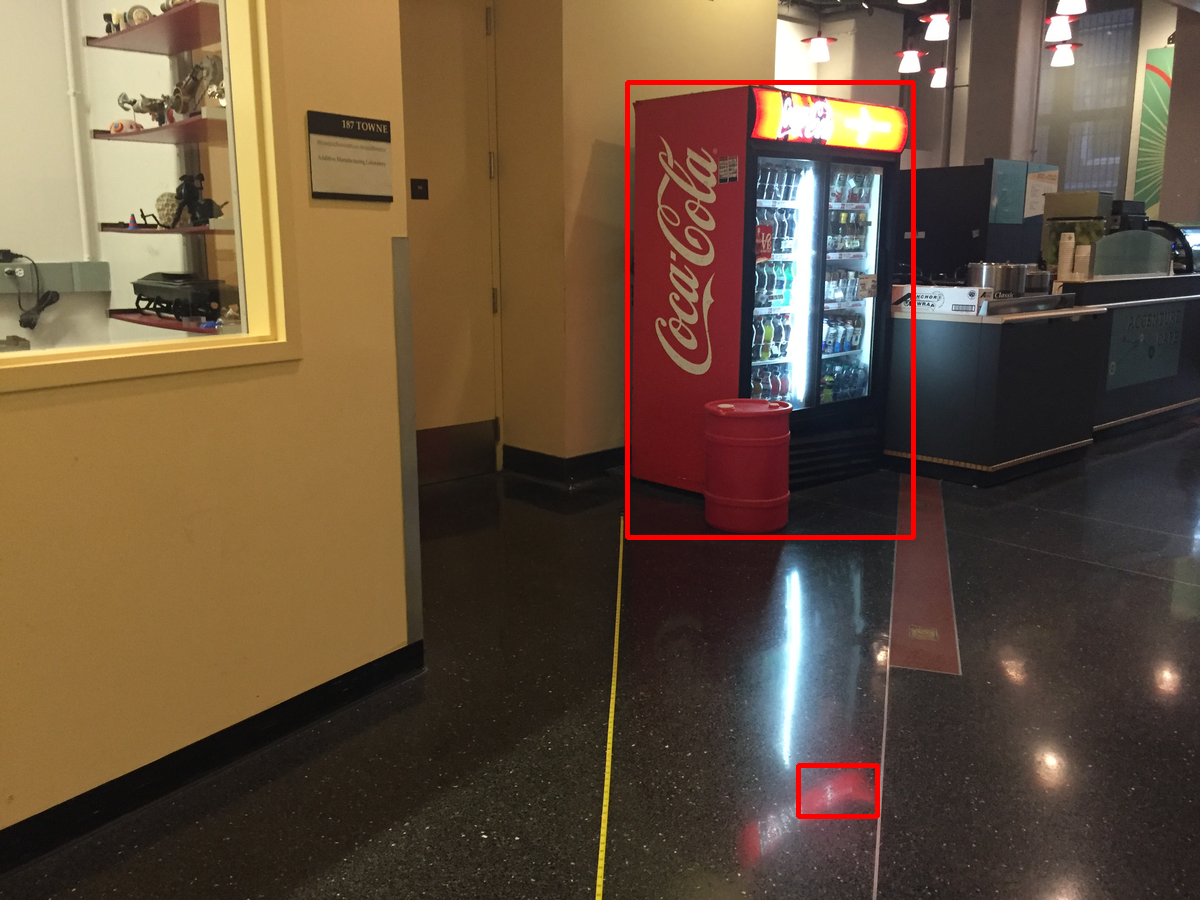
\includegraphics[width=1\textwidth]{test_image2.png}
\caption{\label{fig:test2}Test image 2 result.}
  \end{subfigure}
  \begin{subfigure}[b]{.4\textwidth}
    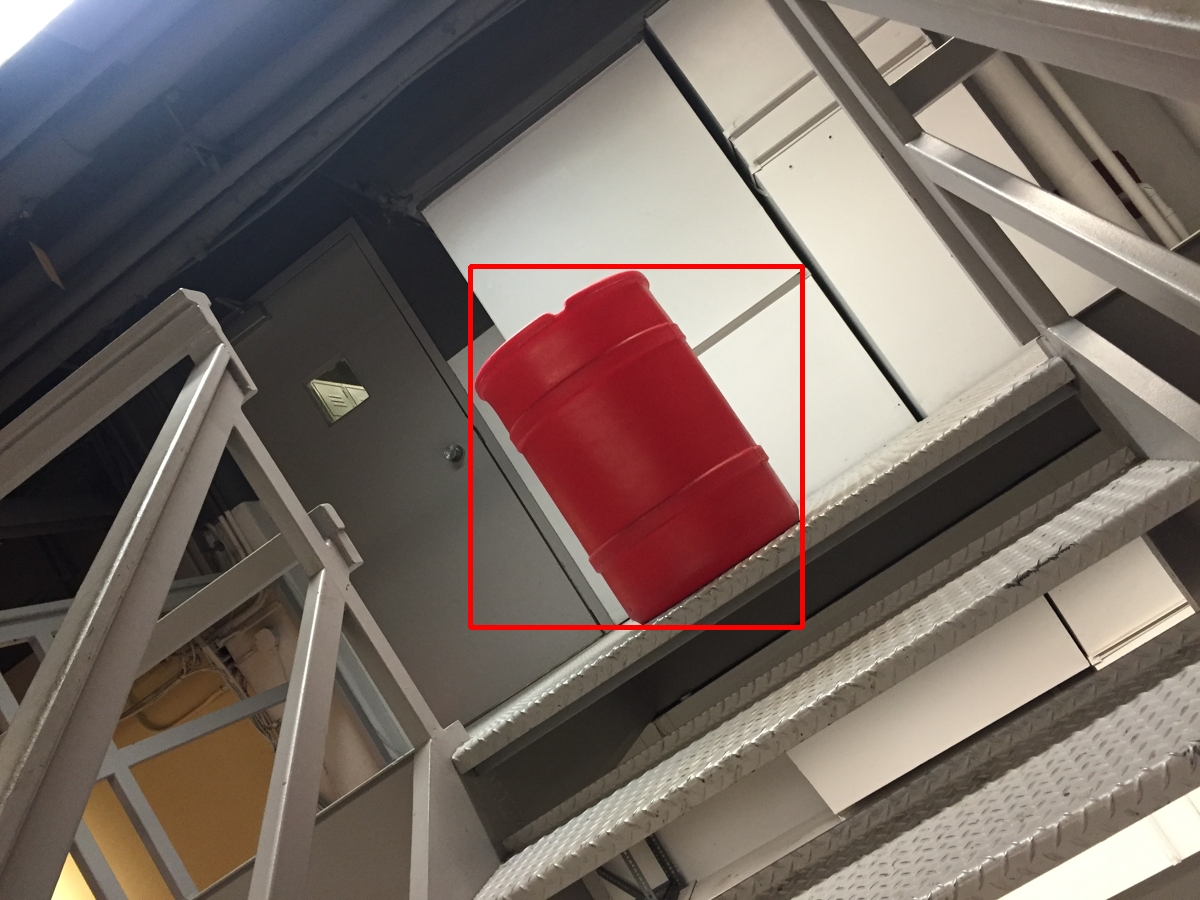
\includegraphics[width=1\textwidth]{test_image3.png}
\caption{\label{fig:test3}Test image 3 result.}
  \end{subfigure}
  \caption{\label{fig:test2_set}}
\end{figure}

\begin{figure}[!tbp]
  \centering
  \begin{subfigure}[b]{.4\textwidth}
    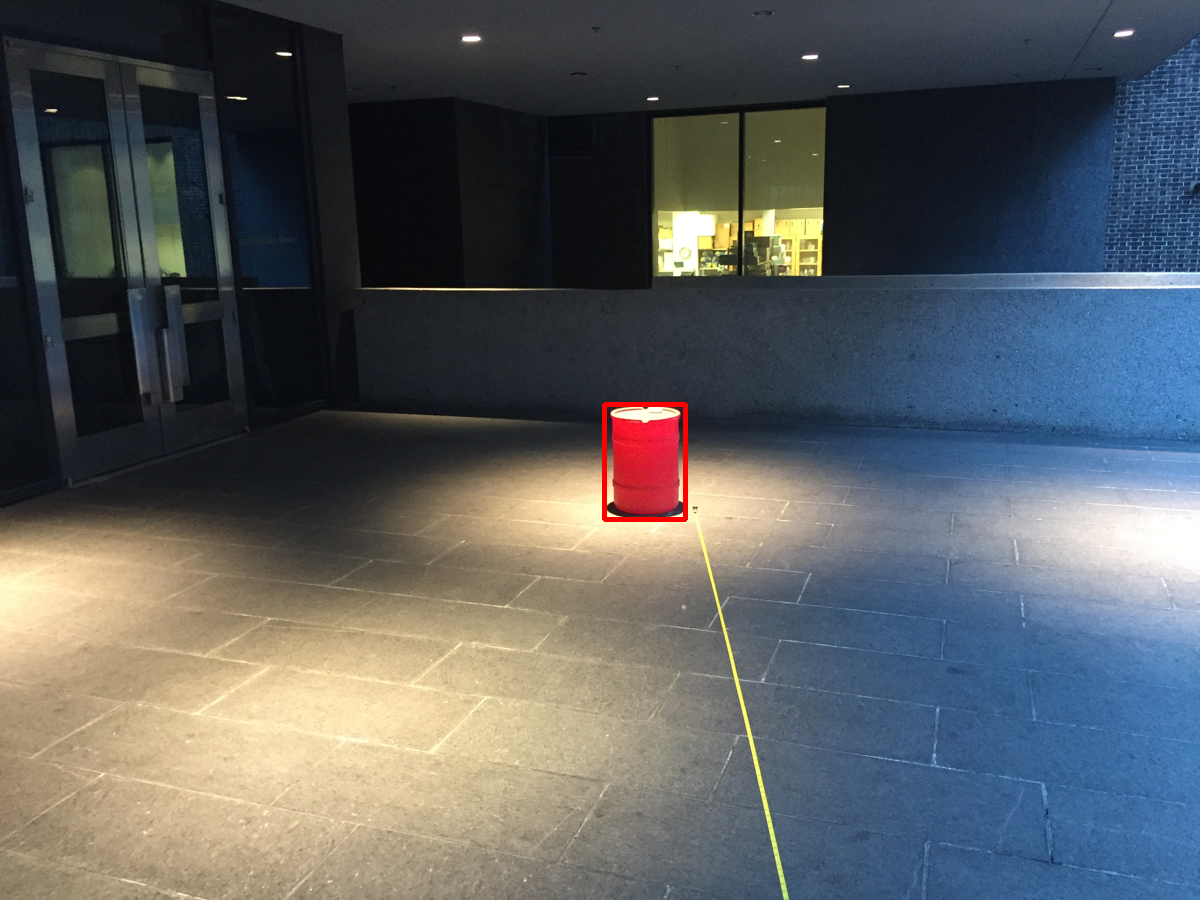
\includegraphics[width=1\textwidth]{test_image4.png}
\caption{\label{fig:test4}Test image 4 result.}
  \end{subfigure}
  \begin{subfigure}[b]{.4\textwidth}
    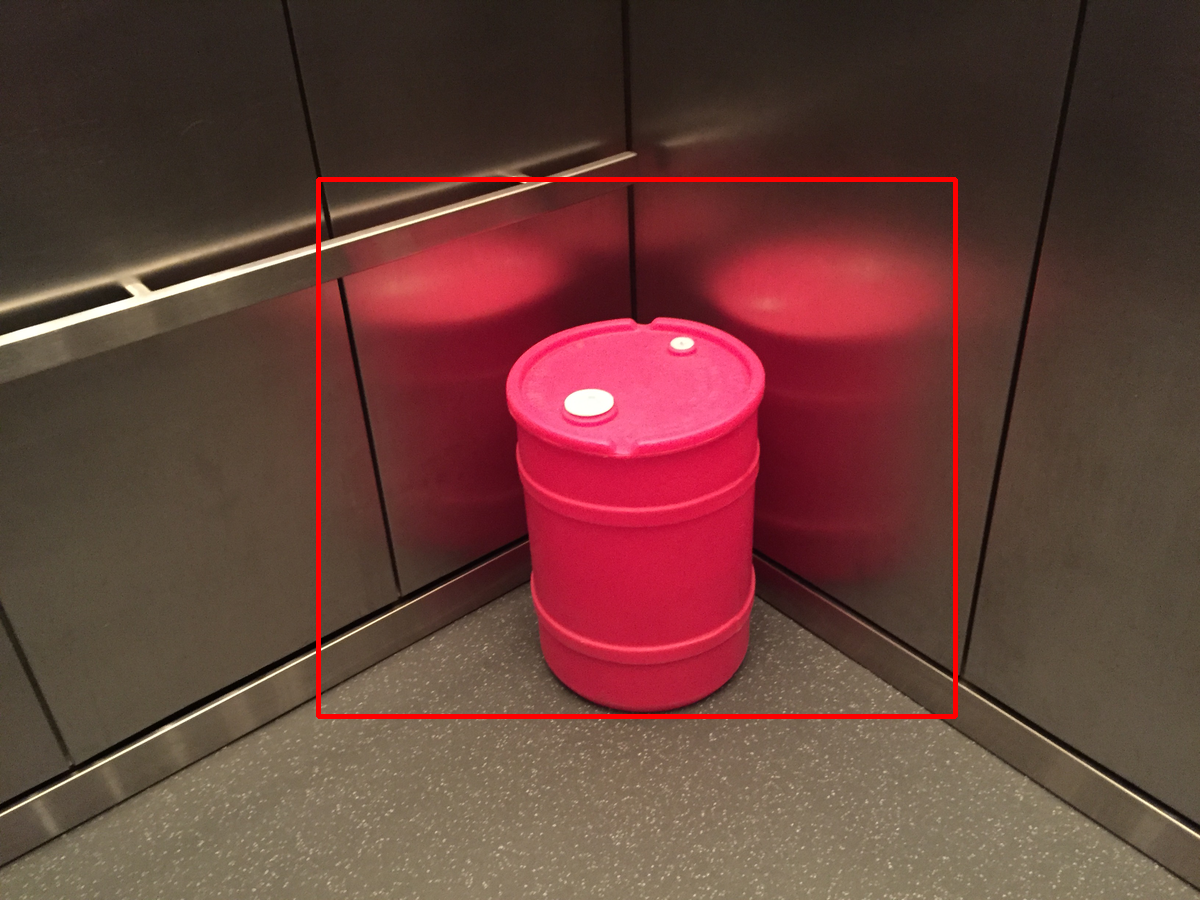
\includegraphics[width=1\textwidth]{test_image5.png}
\caption{\label{fig:test5}Test image 5 result.}
  \end{subfigure}
  \caption{\label{fig:test3_set}}
\end{figure}

\begin{figure}[!tbp]
  \centering
  \begin{subfigure}[b]{.4\textwidth}
    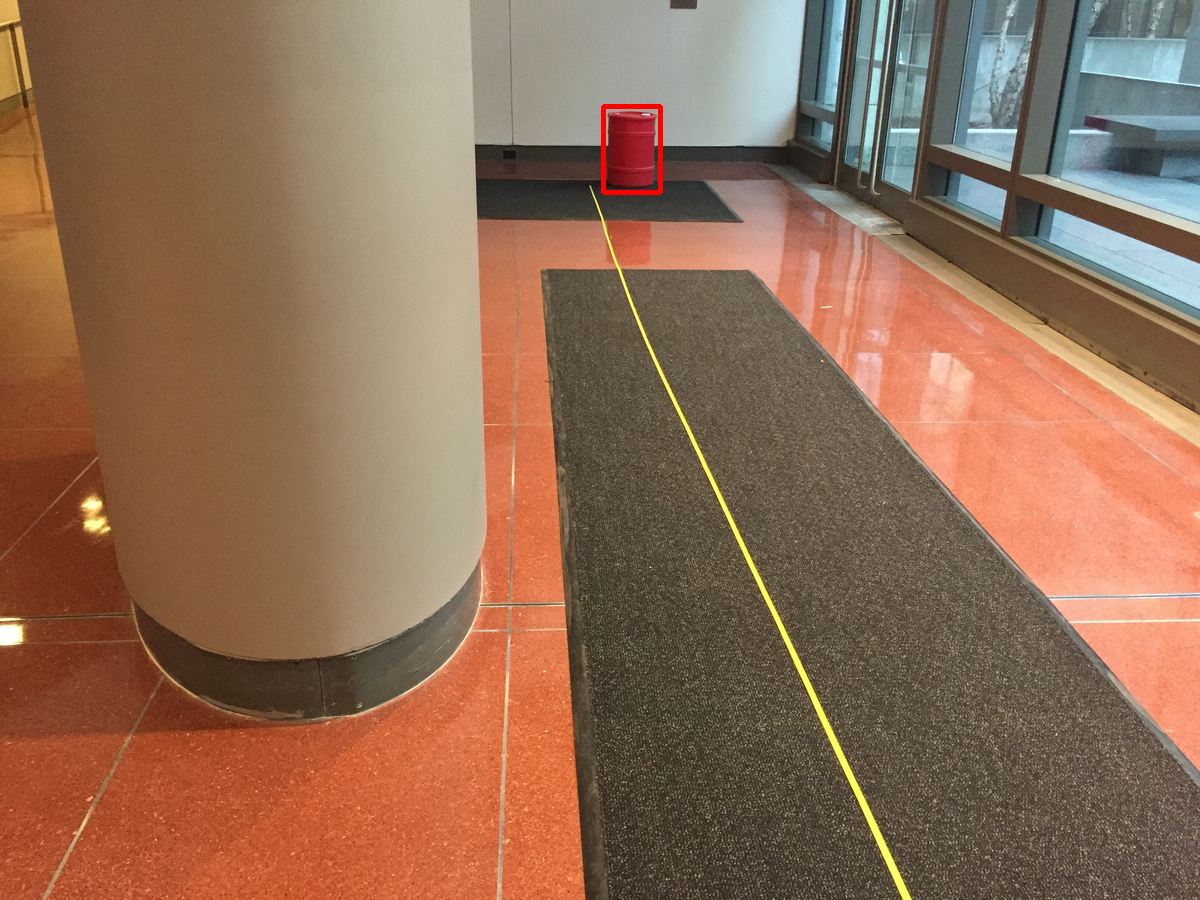
\includegraphics[width=1\textwidth]{test_image6.png}
\caption{\label{fig:test6}Test image 6 result.}
  \end{subfigure}
  \begin{subfigure}[b]{.4\textwidth}
    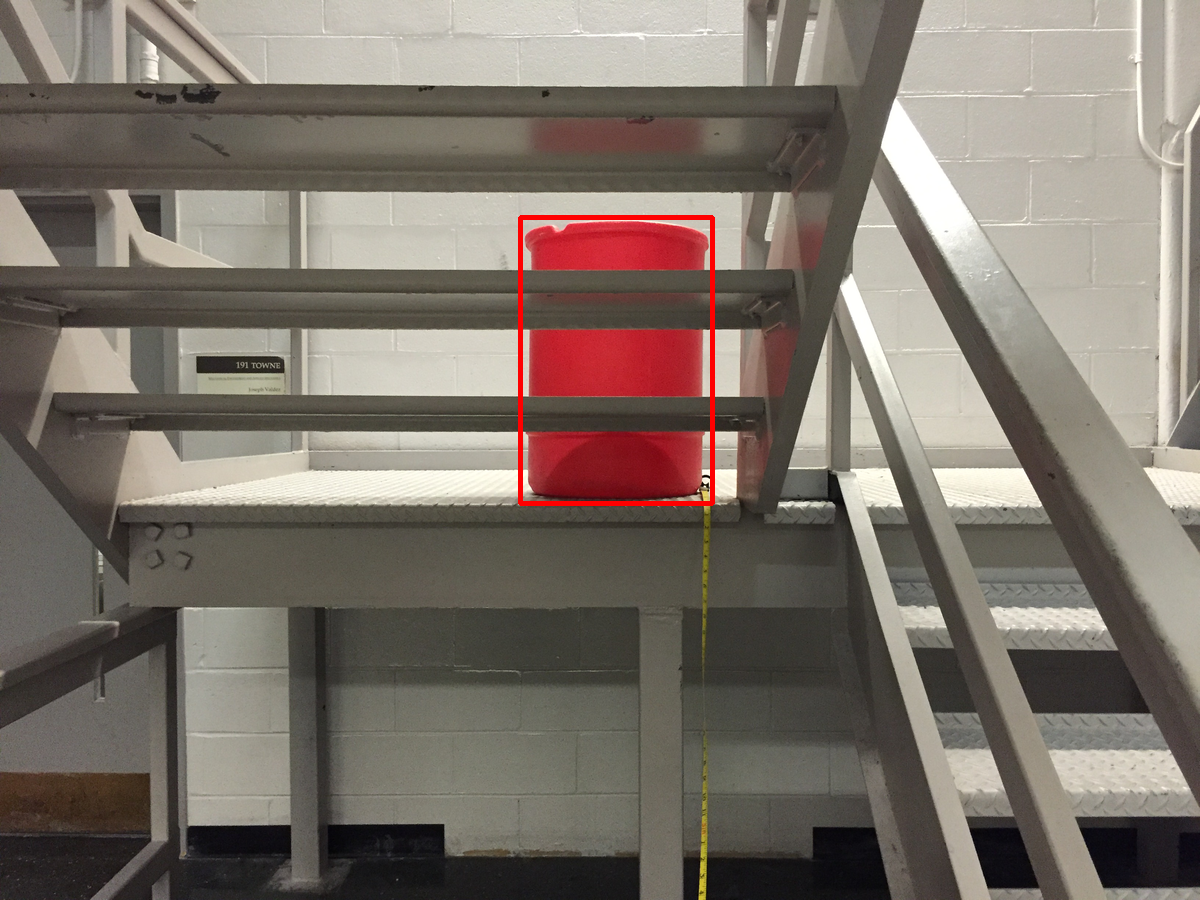
\includegraphics[width=1\textwidth]{test_image7.png}
\caption{\label{fig:test7}Test image 7 result.}
  \end{subfigure}
  \caption{\label{fig:test4_set}}
\end{figure}

\begin{figure}[!tbp]
  \centering
  \begin{subfigure}[b]{.4\textwidth}
    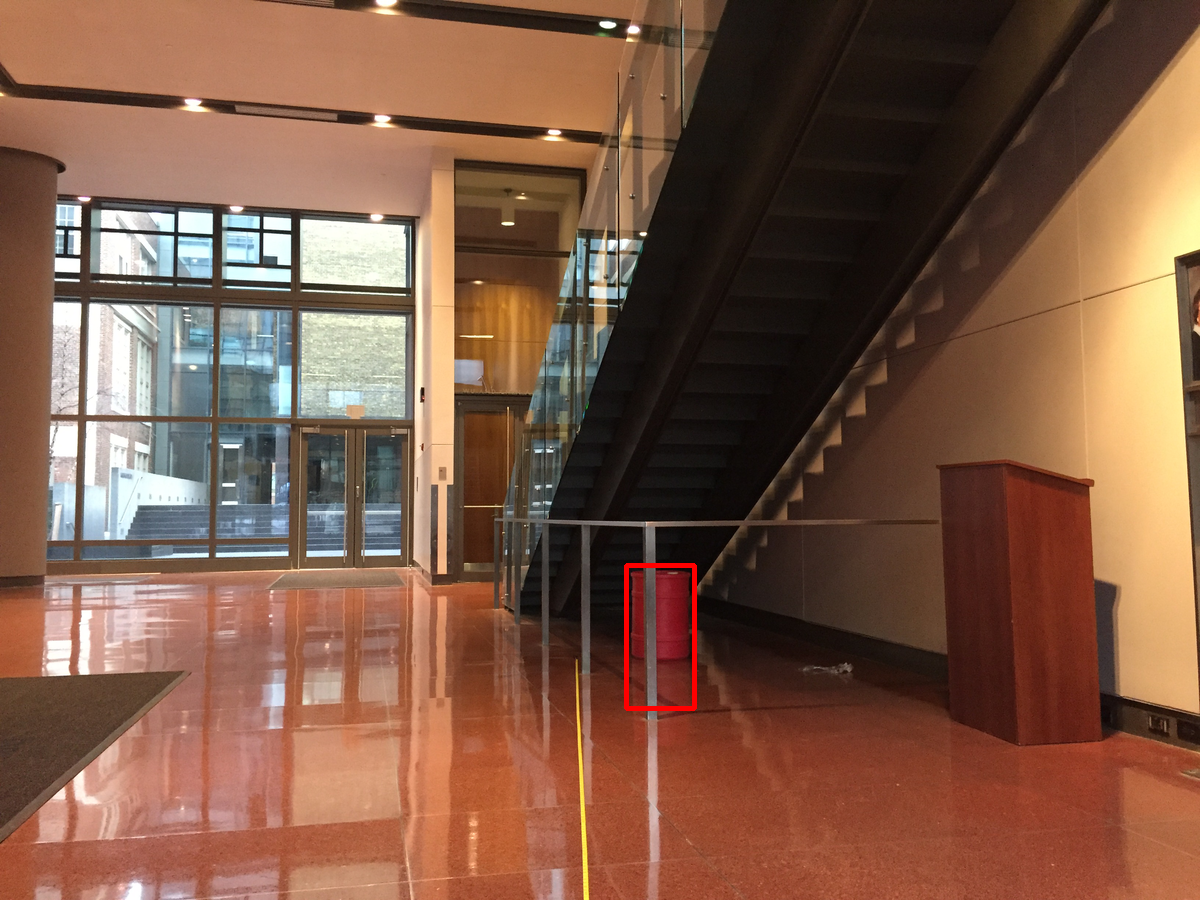
\includegraphics[width=1\textwidth]{test_image8.png}
\caption{\label{fig:test8}Test image 8 result.}
  \end{subfigure}
  \begin{subfigure}[b]{.4\textwidth}
    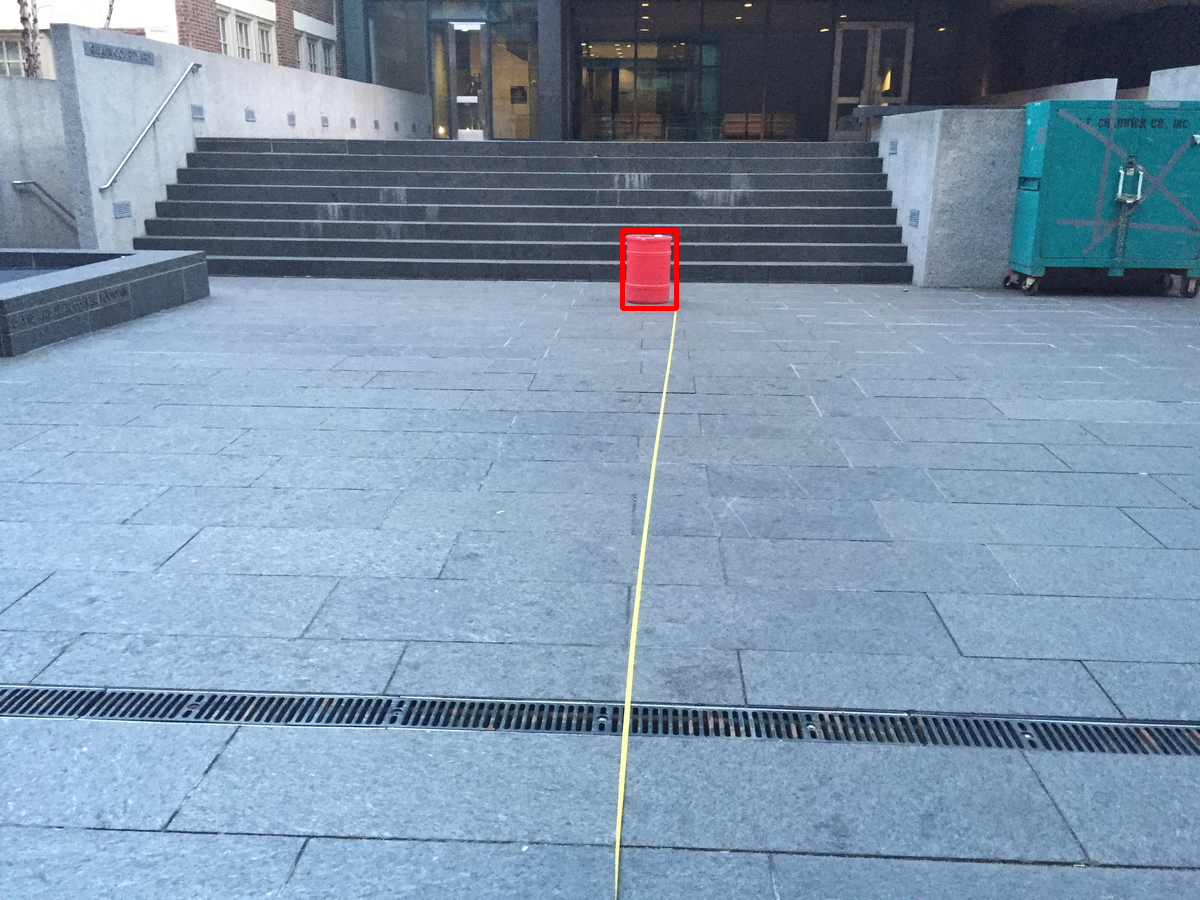
\includegraphics[width=1\textwidth]{test_image9.png}
\caption{\label{fig:test9}Test image 9 result.}
  \end{subfigure}
  \caption{\label{fig:test5_set}}
\end{figure}



\end{document}